\documentclass{stylefiles/capstone}
% This report is adapted from NYUAD CS Capstone Template
\begin{document}

\title{New Yelp Restaurant Rating System}

%year
\capstoneyear{2022}
% options are Seminar, Project 1, Project 2
\capstonedocument{Realtime and Big Data Analysis}
% options are Fall, Spring
\capstonesemester{Spring}

% For each author, provide the names and emails of the students as follows:
\author{Zihao Wang}
\affiliation{%
  \institution{Courant Institute, NYU}
}
\email{zw2486@nyu.edu}

\author{Xiaohan Wu}
\affiliation{%
 \institution{Courant Institute, NYU}
}
\email{xw2788@nyu.edu}

\author{Tianyi Tan}
\affiliation{%
 \institution{Courant Institute, NYU}
}
\email{tt2370@nyu.edu}

\author{Yansong Li}
\affiliation{%
 \institution{Courant Institute, NYU}
}
\email{yl8915@nyu.edu}

% Add your primary advisor's name, then comma-separate all secondary advisors' names.
% Please list advisors only and not secondary graders.
\advisors{Yang Tang}

\renewcommand{\shortauthors}{Wang, Wu, Tan, Li}

\begin{abstract}
  Yelp’s traditional way of rating restaurant lacks of considering the quality of users. Biased, dishonest reviews from low-quality users do more than offset the effects of reviews from objective, honest, high-quality users. In this project, we developed a comprehensive rating system for yelp that included the influence of different quality of users. By referring to reddit’s user rating algorithm, we reasonably assign a rate to each user considering his/her data(friends network, the number of fans, the number of useful, etc). Then we feed the user rate back to the restaurant’s rating process, giving lower weight to low-rate user’s rating and higher weight to high-rate user’s rating vice versa. The final result shows well accomplishment of our designing strategy and objectives. 
\end{abstract}


%Add a list of comma-separated keywords that are relevant to your report. They should be more specific than the list below
\keywords{Big Data, Distributed System, Rating System, MapReduce}



\maketitle

\section{Introduction}
Yelp is a famous review and recommendation mobile application in the United States. On this APP, you can find out how good a restaurant is by checking its rating. However, the rates of the restaurants are oversimplified. It is generally an average of all the stars given by users. If someone uses "zombie accounts" to give reviews on a restaurant, it can greatly affect the rating stars to a unfair, meaningless number. Therefore, we need to avoid such cases by improving the rating algorithms to give a more comprehensive and accurate restaurant rating. 

In our project, we developed a new rating system that takes users quality into account. We believe that an active user with more agreements from other users tends to give a high quality reviews and we should consider more on those kinds of reviews given by a high-quality. To give an improved rating on restaurants on Yelp, we came up with several algorithms on rating users and reviews to re-rating the restaurants. We implemented the algorithms to the Yelp's data on reviews, users, tips, and businesses.

\section{Design Diagrams}
Figure \ref{process_diagram} depicts how we processed the datasets and came up with the final analysis and result. We started with 4 data sources, profiling and cleaning these data in parallel. Then we applied our algorithms to the data and generated the final data. After that, we integrated our processed data with more analysis and computations. At last, we concluded the final results with data visualization.
\begin{figure}[htp]
    \centering
    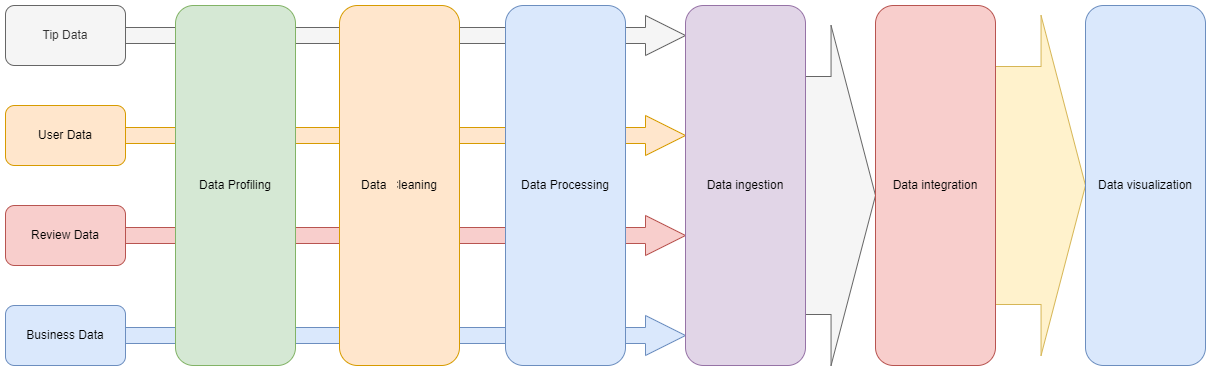
\includegraphics[width=8cm]{asset/Design diagrams-Design Diagram.drawio.png}
    \caption{new rating system architecture}
    \label{process_diagram}
\end{figure}
Figure \ref{system archi} shows the architecture of our new rating system. We implemented our experiments on NYU Peel Cluster. We run MapReduce program on Hadoop and query with Hive and all the data are stored in HDFS inside the Hadoop framework. We also use tableau for visualization to display a vividly result.
\begin{figure}[htp]
    \centering
    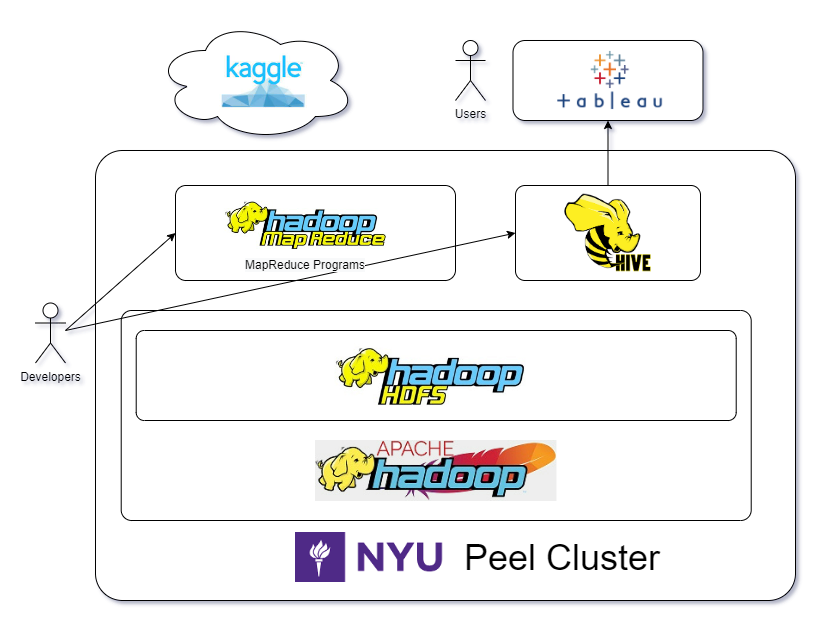
\includegraphics[width=8cm]{asset/Design diagrams-Software Architecture.drawio.png}
    \caption{new rating system architecture}
    \label{system archi}
\end{figure}


\section{Data Sources}
We chose the Yelp dataset\cite{yelpdatasetref} from Kaggle as our source of data. To be more specific, we mainly work on Review, User, Tip and Business data. And the original data are in JSON form. Here shows some details of each dataset.
\begin{enumerate}
    \item Review Data: The formation of Review data is described in Table \ref{ReviewData}. Among the attributes, review\_id, user\_id, business\_id, text and date are string. The number of stars is int. The reactions each review receives like useful, funny, cool and so on are all int.
    \begin{table}[h!]
        \centering
        \begin{tabular}{l r } 
         \hline
         Attribute &  Type \\ [0.5ex] 
         \hline
        review\_id & string\\
        user\_id & string\\
        business\_id & string \\
        stars  &  int\\
        useful  &  int\\
        funny   &  int\\
        cool & int\\
        text & string\\
        date & string\\
         [1ex] 
         \hline
        \end{tabular}
        \caption{Review Data}
    \label{ReviewData}
    \end{table}
    \item User Data
    Review Data: The formation of User data is described in Table \ref{UserData}. Among the attributes, user\_id, name, yelping\_since, elite are string. The number of stars is int. The reactions each user receives like useful, funny, cool are int. And the attribute, friends,which shows the relationship with others of the current user is string.
    \begin{table}[h!]
        \centering
        \begin{tabular}{l r } 
         \hline
         Attribute &  Type \\ [0.5ex] 
         \hline
        user\_id & string\\
        name & string\\
        review\_count & int\\
        yelping\_since & string\\
        useful  &  int\\
        funny   &  int\\
        cool & int\\
        elite & string\\
        friends & string\\
         [1ex] 
         \hline
        \end{tabular}
        \caption{User Data}
    \label{UserData}
    \end{table}
    \item Tip Data: The formation of Tip data is described in Table \ref{TipData}. Among the attributes, user\_id, business\_id, text and date are string. The number of compliment\_count each tip gets is int.
    \begin{table}[h!]
        \centering
        \begin{tabular}{l r } 
         \hline
         Attribute &  Type \\ [0.5ex] 
         \hline
        user\_id & string\\
        business\_id & string\\
        text & string\\
        date & string\\
        compliment\_count & int\\
         [1ex] 
         \hline
        \end{tabular}
        \caption{Tip Data}
    \label{TipData}
    \end{table}
    
    \begin{table}[h!]
        \centering
        \begin{tabular}{l r } 
         \hline
         Attribute &  Type \\ [0.5ex] 
         \hline
        business\_id & string\\
        name & string\\
        address & string\\
        city & string\\
        postal\_code & string\\
        latitude & float\\
        longitude & float\\
        stars & int\\
        review\_count & int\\
        is\_open & int\\
        ByAppointmentOnly & string\\
        categories & string\\
         [1ex] 
         \hline
        \end{tabular}
        \caption{Business Data}
    \label{BusinessData}
    \end{table}
    \item Business Data: The formation of Tip data is described in Table \ref{BusinessData}. Among the attributes, business\_id and name are string. The information about location like address, city, postal\_code are string. What is more, latitude and longitude are provided as float. And stars, review\_count are int. Is\_open and ByAppointmentOnly are int and string respectively to indicate true and false. Finally, the business are categorized with categories, which is string.
\end{enumerate}


\section{Data Pre-processing}
\subsection{Data Profiling}
\subsubsection{\textbf{Review}}

In Review Data Profiling, we counted the lines of available data and checked if the data exceeded the maximum or minimum boundary of each columns. A MapReduce program is written for profiling the review data. Here is a brief description of the main components:

\textbf{Mapper}.
\texttt{ReviewMapper} ~is the mapper for review data profiling. It reads the data in String, tailors data into txt format by removing punctuation marks. We also checked if fields stars, useful, funny, and cool are out of boundary. The output key for the mapper is the field name and the output value is a \texttt{Text}. 

\textbf{Reducer}.
\texttt{ReviewReducer} is the reducer for review data profiling. It reads the data in the form of mapper's output form which is a key-value pair of <Text, Text>. Since we checked the outlier data on the mapper side, we can compute the sum for each field and observe if they are all equal in the reducer side. Note that if the count of any field in [stars, useful, funny, and cool] is less than the count of field review\_id, then there is ourlier. We output the count of all fields as final result for profiling.

\textbf{Output}.
Table \ref{review_profile_table} shows the output of the review data profiling. Observe that each field in review Data has 6990280 lines, therefore there is no outlier and each field's range conform to their own definition. Overall, The result of review data profiling meets the expectation.

\begin{table}[h!]
\centering
\begin{tabular}{l r r r} 
 \hline
 Fields &  Count \\ [0.5ex] 
 \hline
business\_id    &      6990280 \\
cool  &  6990280\\
date  &  6990280\\
funny    &       6990280\\
review\_id   &    6990280\\
stars  &  6990280\\
text  &  6990280\\
useful  &  6990280\\
user\_id      &    6990280\\
 [1ex] 
 \hline
\end{tabular}
\caption{Review data profiling output}
\label{review_profile_table}
\end{table}

\subsubsection{\textbf{User}}

In User Data Profiling, we counted the lines of available data and computed the maximum and minimum of each columns. A MapReduce program is written for profiling the user data. Here is a brief description of the main components:

\textbf{Tuple}.
\texttt{UserProfilingTuple}is a custom class created for transferring multiple values in a package. The class contains 4 members. \texttt{max}, \texttt{min}, and \texttt{count} are \texttt{double} type variables to save the maximum, minimum, and counting number of each field. \texttt{isUserId} is \texttt{Boolean} type. If \texttt{isUserId} is \texttt{False}, \texttt{UserProfilingTuple} is for profiling a field. If it is \texttt{True}, it is used to count if there is any duplicate lines for a same user ID because user ID is our primary key for the user table, we need to make sure it is unique.

\textbf{Mapper}.
\texttt{UserProfilingMapper} ~is the mapper for user data profiling. It reads the data in String, converts the data into a Java object based on class \texttt{User}. In the class, members are declared based on the source data. There are 22 fields in total, covering data type int, double, and String. We handle each of the fields respectively according to our needs. For number types, we simply initialized 1; for date type, we converted it into timestamp; and for lists, we initialized with the number of elements in the list. The output key for the mapper is the field name or a user ID and the output value is a \texttt{UserProfilingTuple}. The reason We also generate pairs with user ID is that we need to ensure that there is no duplicate user ID.

\textbf{Reducer}.
\texttt{UserProfilingReducer} is the reducer for user data profiling. It reads the data in the form of mapper's output form which is a key-value pair of <Text, UserProfilingTuple>. Since we have handled data on the mapper side, we only need to compute the maximum and the minimum and sum up the count for each field and output the final result for profiling.

\textbf{Output}.
Table \ref{user_profile_table} shows the output of the user data profiling. User Data has 1987897 lines of data and the ranges all conform to their definition. Overall, The result of user data profiling meets the expectation.

\begin{table}[h!]
\centering
\begin{tabular}{l r r r} 
 \hline
 Fields & Max & Min & Count \\ [0.5ex] 
 \hline
average\_stars    &      5.0    &    1.0  &  1987897 \\
compliment\_cool  &  49967.0    &    0.0   & 1987897\\
compliment\_cute  &  13654.0     &   0.0   & 1987897\\
compliment\_funny    &       49967.0     &   0.0  &  1987897\\
compliment\_hot   &  25784.0   &     0.0  &  1987897\\
compliment\_list  &  12669.0   &     0.0  &  1987897\\
compliment\_more  &  13501.0   &     0.0  &  1987897\\
compliment\_note  &  59031.0  &      0.0  &  1987897\\
compliment\_photos      &    82630.0   &     0.0  &  1987897\\
compliment\_plain      &    101097.0  &      0.0   & 1987897\\
compliment\_profile      &   14180.0     &   0.0   & 1987897\\
compliment\_writer      &    15934.0    &    0.0  &  1987897\\
cool   &   199878.0    &    0.0  &  1987897\\
elite    &      0.0    &    0.0  & 1987897\\
fans    &   12497.0     &   0.0  &  1987897\\
friends  &  14995.0    &    0.0  &  1987897\\
funny   &  185823.0    &    0.0  &  1987897\\
name   &        0.0     &   0.0  &  1987897\\
review\_count    &   17473.0     &   0.0   & 1987897\\
useful  &  206296.0     &   0.0   & 1987897\\
user\_id    &    0.0     &   0.0   & 1987897\\
 [1ex] 
 \hline
\end{tabular}
\caption{User data profiling output}
\label{user_profile_table}
\end{table}

\subsubsection{\textbf{Tip}}

Firstly, we used MapReduce to take a whole view of the Tip Dataset, where we calculate the max and min values of each attribute and count the number of records. 

\textbf{Mapper}. For user\_id, business\_id, date and text, these data are in string type, so we set the max and min to zero and set count to one (Because it is overview here, we do not need to pay much attention to their values). For compliment\_count, I find out the max and min value with Mapper and Reducer. 

\textbf{Reducer}. We compare the max of value with the current value and pick the greater one. And it is the same case with min. As to count, we added the ones up and get the results.

And the results (as shown in Table \ref{tip_overview}, which corresponds to max, min and count in order) of MapReduce show that there are 908915 records in all in Tip Dataset. What worth mentioning is that the max value and min value of compliments are all zero in Tip Dataset, which means compliment offers little help to our analysis.

\begin{table}[h!]
\centering
\begin{tabular}{l r r r} 
 \hline
 Fields & Max & Min & Count \\ [0.5ex] 
 \hline
user\_id &  0.0 & 0.0 &  908915 \\
business\_id  &  0.0 &  0.0 &  908915\\
date &  0.0  &  0.0  &  908915\\
text &  0.0  &  0.0  &  908915\\
compliment\_count  &  0.0 &  0.0  &  908915\\
 [1ex] 
 \hline
\end{tabular}
\caption{Overview of Tip data}
\label{tip_overview}
\end{table}

Based on the results of overview, we decide to ignore compliment and turn to analyze the length of user\_id, business\_id, text and date. To be more specific, we calculate the maximum length and minimum length and make counts. Also, we pay attention to the sum of the length of attributes in all records, thus finding out the average length.

For max, min and count, it is the same as in Data Whole Viewing. For sum and average, we set it to the value itself in the Mapper add them up in the Reducer. For average, we set it to zero in the Mapper and calculate it with sum and count in the Reducer.
As the results (Table \ref{tip_analysis}, which corresponds to max, min, sum count and average in order) show, user\_id, business\_id and date are all in good form and each record has the same length in these three attributes. As to text, its length ranges from 5 to 204 and the average length is 53, indicating good validity. (Since the data profiling make improvements based on data whole viewing, we directly put the code of data profiling in submission.)


\begin{table}[h!]
\centering
\begin{tabular}{l r r r r r} 
 \hline
 Fields & Max & Min & Sum & Count & Average \\ [0.5ex] 
 \hline
user\_id &  22 & 22 & 19996130 & 908915 & 22\\
business\_id  & 22 & 22 & 19996130 & 908915 & 22\\
date &  19  &  19 & 17269385 &  908915 & 19\\
text &  500  &  1  &  56880106 & 908915 &62\\
 [1ex] 
 \hline
\end{tabular}
\caption{Overview of Tip data}
\label{tip_analysis}
\end{table}

\subsubsection{\textbf{Business}}


The whole business dataset contains 150346 recordings of data. There is no duplicating data in this dataset as every business\_id in this dataset is unique. However, after necessary steps of data cleaning, there is only 64703 recordings of data left. 


The columns of business dataset include business\_id, name, address, city, state, postal\_code, latitude, longitude,  stars, review\_count, is\_open, attributes, categories and hours. We did related mapreduce programming for some specific columns. As mentioned above, first, we checked whether all the business\_id is unique. Then we get the profiling of state column. The result is shown in the Table \ref{business_state_count_analysis}. The result shows that some states have few data while some states have much data. Those states which have small amounts of data are trivial to data analysis. Thus, we decided to remove data related to these states. The result is shown in the Table \ref{business_state_count_after_filter_analysis}. To clarify, the result shown in the Table \ref{business_state_count_after_filter_analysis} is generated after other cleaning steps. 

Then, we did mapreduce programming for the column is\_open to check how many businesses are still open. All the business which are not open is filtered in data cleaning part.

\begin{table}[h!]
\centering
\begin{tabular}{l r r r r r} 
 \hline
 State & Count \\ [0.5ex] 
 \hline
MI & 1 \\
MT & 1 \\
NC & 1 \\
SD & 1 \\
UT & 1 \\
VI & 1 \\
VT & 1 \\
XMS & 1 \\
HI & 2 \\
MA & 2 \\
WA & 2 \\
CO & 3 \\
TX & 4  \\
IL & 2145 \\
DE & 2265 \\
ID & 4467 \\
CA & 5203 \\
AB & 5573 \\
NV & 7715 \\
NJ & 8536 \\
AZ & 9912  \\
LA & 9924 \\
MO & 10913 \\
IN & 11247 \\
TN & 12056  \\
FL & 26330 \\
PA & 34039 \\
 [1ex] 
 \hline
\end{tabular}
\caption{Overview of Business State Statistics}
\label{business_state_count_analysis}
\end{table}

\begin{table}[h!]
\centering
\begin{tabular}{l r r r r r} 
 \hline
 State & Count \\ [0.5ex] 
 \hline
CA & 1659  \\
ID & 1754  \\
NV & 2404  \\
AB & 3058  \\
AZ & 3460  \\
NJ & 4200  \\
LA & 4879  \\
IN & 5291  \\
MO & 5311  \\
TN & 5478  \\
FL & 11283  \\
PA & 15926 \\
 [1ex] 
 \hline
\end{tabular}
\caption{Overview of Business State Statistics After Cleaning}
\label{business_state_count_after_filter_analysis}
\end{table}


Then we did MapReduce programming for the column attributes. As our focus of the data analysis is mainly about restaurants business. The profiling of attributes is shown in the table below. It turns out that this dataset contains much data not related to restaurants. Part of the result is shown in the Table \ref{business_category_count_analysis}. The result shows that these businesses belong to a large number of sub categories in the service industry. So we decided to filter out businesses which don't belong to restaurant industry. Part of the result is shown in the Table \ref{business_category_count_analysis_after_cleaning}.

\begin{table}[h!]
\centering
\begin{tabular}{l r r r r r} 
 \hline
 Category & Count \\ [0.5ex] 
 \hline
Food &	27781  \\
Shopping &	24395 \\
Home Services &	14356 \\
Beauty Spas &	14292 \\
Nightlife &	12281 \\
Health Medical &	11890 \\
Local Services &	11198 \\
Bars &	11065 \\
Automotive & 10773 \\
Event Planning  Services &	9895 \\
Sandwiches &	8366 \\
American (Traditional) &	8139 \\
Active Life &	7687 \\
Pizza &	7093 \\
Coffee Tea &	6703 \\
Fast Food &	6472 \\
Breakfast Brunch &	6239 \\
American (New) &	6097 \\
Hotels Travel &	5857 \\
Home Garden &	5799 \\
 [1ex] 
 \hline
\end{tabular}
\caption{Overview of Business Category Statistics After Cleaning}
\label{business_category_count_analysis_after_cleaning}
\end{table}

Finally, we need to get the statistics of reviews. We did MapReduce programming to get the distribution of review count. The result is shown in the Table \ref{}. It turns out most business have fewer than 100 reviews while the business which has top 1 review count has over 3500 reviews. 

\begin{table}[h!]
\centering
\begin{tabular}{l r r r r r} 
 \hline
 Review Description & Count \\ [0.5ex] 
 Review count between 0 and 50 &	11606  \\
Review count between 50 and 100	& 1793  \\
Review count between 100 and 150 &	605 \\
Review count between 150 and 200 & 	289 \\
Review count between 200 and 250 & 	159 \\
Review count between 250 and 300 & 	104 \\
Review count between 300 and 350 & 	71 \\
Review count between 350 and 400 & 	42 \\
Review count between 400 and 450 & 	28 \\
Review count between 450 and 500 & 	23 \\
Review count between 500 and 550 & 	19 \\
Review count between 550 and 600 & 	12 \\
Review count between 600 and 650 & 	11 \\
Review count between 650 and 700 & 	10  \\
Review count between 700 and 750 & 	10 \\
Review count between 750 and 800 & 	8 \\
Review count between 800 and 850 & 	3 \\
Review count between 850 and 900 & 	2 \\
Review count between 900 and 950 & 	4 \\
Review count between 950 and 1000 &  5  \\
Review count between 1000 and 1050 & 	2  \\
Review count between 1150 and 1200 & 	3 \\
Review count between 1200 and 1250 & 	1 \\
Review count between 1350 and 1400 & 	1 \\
Review count between 1400 and 1450 & 	1 \\
Review count between 1450 and 1500 & 	1 \\
Review count between 1500 and 1550 & 	1 \\
Review count between 1600 and 1650 & 	1 \\
Review count between 1850 and 1900 & 	1 \\
Review count between 1900 and 1950 & 	1 \\
Review count between 2050 and 2100 & 	3 \\
Review count between 2400 and 2450 & 	1 \\
Review count between 3150 and 3200 & 	1 \\
Review count between 3400 and 3450 & 	1 \\
 [1ex] 
 \hline
\end{tabular}
\caption{Overview of Business Review Statistics}
\label{business_review_count_analysis}
\end{table}

\subsection{Data Cleaning}
\subsubsection{\textbf{Review}}

In the review data cleaning, as review dataset shares the business\_id column with business dataset, we filtered the review data according to filtered business data. Taking review and business dataset as multiple input, we wrote two mapper classes. The processed data sent from two mappers shared the business\_id as key. The reducer thus is able to filter out review which doesn't have related business. 

\subsubsection{\textbf{User}}

In User Data Cleaning, we dropped columns: name and elite and reformatted user source data to be readable data for Hive.

\textbf{Tuple}.
\texttt{UserCleaningTuple} is the custom class created for transferring data which contains the fields of User that are needed for later analysis. We override the write methods to format the output as required for Hive, splitting each field with semicolon.

\textbf{Mapper}.
\texttt{UserCleaningMapper} is the mapper for user data cleaning. It reads and converts source data into a Java object in the same way in profiling User data. Mapper here is for dropping the columns that will not be involved in the later analysis.

\textbf{Reducer}.
We didn't use a Reducer for the Data cleaning.

\textbf{Output}.
Table \ref{user_clean_table} shows a 5-line snippet of the output of the user data cleaning selected from Hive. All the User data are stored in Hive now.
\begin{table}[h!]
\centering
\begin{tabular}{llll} 
 \hline
user\_id & review & fans & stars   \\ [0.5ex] 
 \hline
$ eAw1TQ-FCrPmlgYYkG-ahg $ & 116 & 19 & 4.22 \\
$ fVCZpM3qg7pgbnVPfEmYJQ $ & 100 & 17 & 4.23  \\
$ o5PjjS1IxZ8rvBKSFZeM7Q $ & 665 & 105 & 3.96  \\
$ MvzUoye4DKsBdB4dylgpDw $ & 53 & 17 & 3.99  \\
$ RkgwgvTEu9BkHjEcOOP7MA $ & 136 & 14 & 4.15  \\
 \hline
\end{tabular}
\caption{User data profiling output}

\label{user_clean_table}
\end{table}

\subsubsection{\textbf{Tip}}
Considering the Tip dataset is in JSON form, to better organize it, we use MapReduce to clean and reconstruct. We extract useful information from the JSON file and discard the redundant characters of JSON. We keep the original form of user\_id, business\_id and data. As to text, we replace the text content with the length of text, thus making it more excusable. And we use “;” as the delimiter. In this process, Reducer is unnecessary, and the output is generated by the Mapper. And the results are like shown in Fig \ref{tipclean}.

\begin{figure}[htbp]
\centering
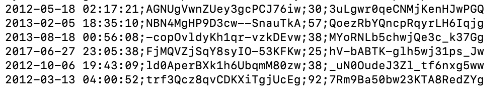
\includegraphics[width=0.48\textwidth]{asset/tipclean.png}
\caption{Result of Tip cleaning}
\label{tipclean}
\end{figure}
\subsubsection{\textbf{Business}}
Steps of business dataset cleaning are designed according to statistics calculated in the profiling step. As mentioned before, we did several steps of business data cleaning. First, we removed states which have few businesses. Then, we filtered out businesses which don't belong to the restaurant industry. Then, we found that only open businesses are useful to business analysis. So we removed all the business data which are not open. Last but not least, all the columns which we won't use in the future analysis are discarded such as longitude and hours.

\section{Data Processing}
\subsection{User re-Rating}\label{user_rerating}
\subsubsection{\textbf{Algorithm}}
Assume that we have a user $u$, we denote the number of reviews $u$ receives as $N$. Also, the number of reactions like `useful', `cool' and so on is denoted by $V$. $F$ represents the number of friends $u$ has. $T$ means the time since $u$ has become a Yelp user. $G$ is the time factor, which is 1.3 here. We would firstly give the equation that we use to re-rate the weight of users in Equ \ref{user_rerate}:
\begin{equation}
weight_{re-rate}=1+\log_{10}{\frac{V}{N+1}*\frac{\log_{10}F}{(T+1)^{-G}}}
\label{user_rerate}
\end{equation}
To further explain the equation: The part of $\frac{V}{N+1}$ shows that the more positive reactions a user’s per review get, the more important a user is. As to $\log_{10}F$, we refers to the mechanism that Reddis takes \cite{redditref} to handle the number of user's friends: The more friends a user has, the more influence he/she could exert. However, the change rate of should gradually slow downs, which follows the  trend of function $\log$. And $(T+1)^G$ plays the role of deciding that the longer a user joins yelp, the more senior he/she may be and $G$ would decide the change rate of time $T$. 

With the novel rating mechanism, the weights of users range from 1 to 20. After adjusting the user rating. The stars each restaurant retains maps from the original [0,5] to [0,100] now, which provides a more specific rating system and could help customers better differentiate the restaurants, thus making their own choice.

\subsubsection{\textbf{Implementation}}
The above algorithms are implemented with MapReduce within the data processing step after cleaning the data. The algorithm is implemented in Mapper and the computation result is saved into a custom tuple along with some other immediate variables. The exact value of $G$ we have mentioned in \ref{user_rerate} is decided by hundreds of experiments to ensure that the final outcome of user rates will fall into a range from 1 to 20. An example is given below:
\begin{table}[h!]
\centering
\begin{tabular}{llllll} 
 \hline
username & review & rate & friends & fans & average\_stars   \\ [0.5ex] 
 \hline
$ User1 $ & 3315 & 18.16 & 11026 & 1124 & 3.77  \\
$ User2 $ & 789 & 17.78 & 10366 & 283 & 3.86  \\
 \hline
\end{tabular}
\caption{User re-rate output example}

\label{user_rerating_output}
\end{table}
Table \ref{user_rerating_output} shows an example of the output of the user re-rating algorithm. Originally, the average\_stars of User1 is less than that of User2. However, since User1 has more fans and has far more reviews than User2, it is reasonable to consider User1 has a higher quality than User2, or User1 is more likely to give a high quality review than User2. Clearly, the original rating algorithm doesn't take those into account. On the contrary, the User re-rating algorithm in our project is able to discover these important factors and show the differences in the re-rating result. Thus, we can see that the rate of User1 is 18.16 which is higher than the 17.78 rate of User2.


\subsection{Business re-Rating}
\subsubsection{Algorithm}
As we mentioned in \ref{user_rerating}, we need to add up the stars of restaurants with users' weights and we also take into account the number of review\_count of each restaurant since the number ranges from dozens to thousands. The following Equ \ref{review_weight} gives the equation based on the number of reviews for each restaurant.  

\begin{equation}
weight_{review}= log_{10}(\frac{review_count}{3.5}+1)
\label{review_weight}
\end{equation}

\subsubsection{Implementation}
To implement the algorithm above, first we added the adjusted user stars to each review created by the user. Then we joined two datasets review and business. We implemented two Mapper classes respectively to process review and business datasets. Then we collected the data processed by the Mapper and implemented the algorithm in the reducer. The data sent from those two Mapper classes share the same business id. Thus we can get the review count of each business and calculate the weight of this review count. By multiplying the adjusted review stars and weight of the business, we got the adjusted rate for the business.
\section{Data Integration}

First, we integrated the user and review datasets as both datasets share the review\_id column. In the algorithm above, we need to adjust the review stars according to new user stars as we suggest that user is able to affect the quality of his/her reviews. By joining these two datasets together, we added a new column to review dataset for later analysis. 

Then, we joined the business and review dataset together as our final goal is to adjust the stars for all the business. Each review could affect the stars of the business, so does the count of review. The review and business datasets share the same column: business\_id. By joining the two datasets together, we could easily implement the algorithm of re-rating business stars. 

In summary, by integrating related datasets, we could do further analysis on yelp business data. The data integration helped us realize the initial idea and implement the analysis pipeline of big data.

\section{Data visualization}

\begin{figure}[htp]
    \centering
    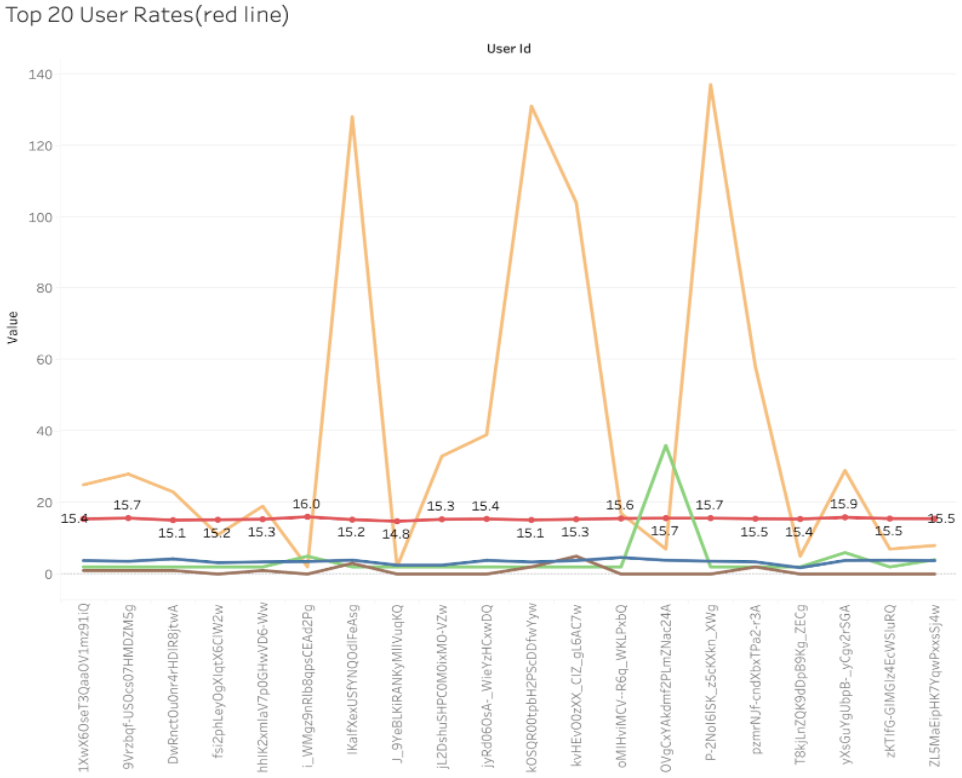
\includegraphics[width=8cm]{asset/result_1.png}
    \caption{User rates (red line) and user data}
    \label{line_chart_figure}
\end{figure}

Figure \ref{line_chart_figure} shows a line chart of the user rates and user data.
The red line shows the rate for top 20 users. Other lines are user data we considered in minting the user rate. They are Review Count (yellow line), Friends (green line), Fans (grey line), Average Stars (blue line), respectively.

\begin{figure}[htp]
    \centering
    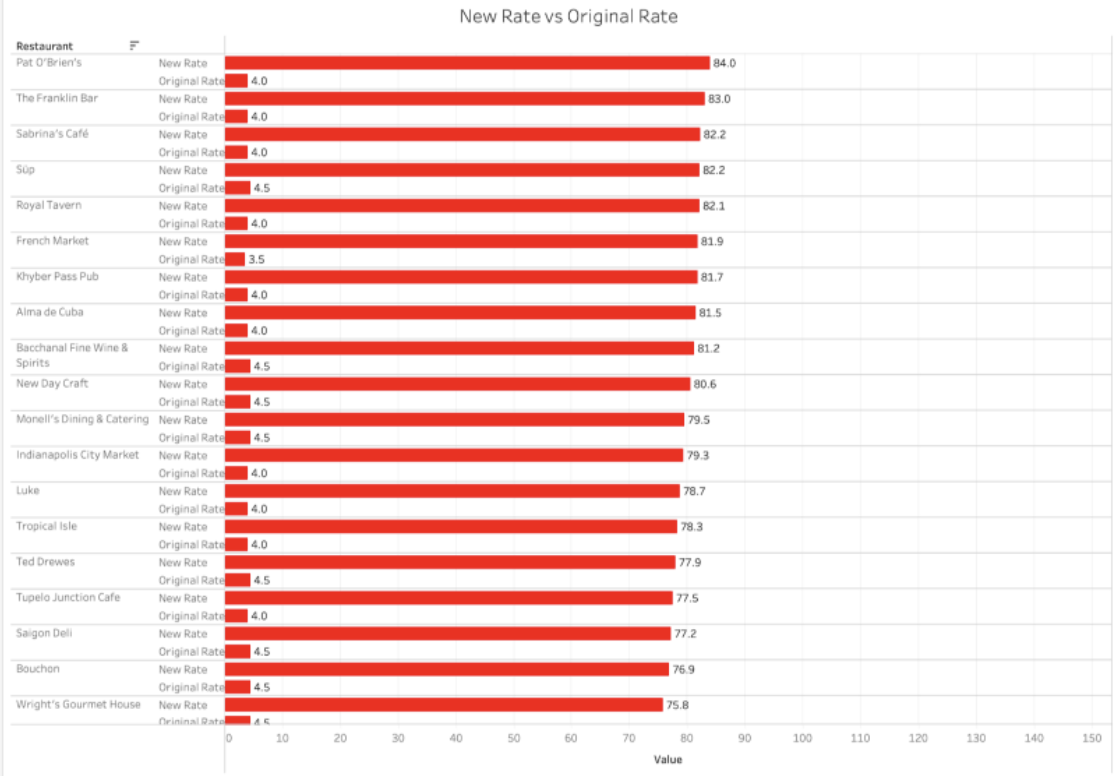
\includegraphics[width=8cm]{asset/result_2.png}
    \caption{New Rate vs Original Rate}
    \label{rate_comparasion_figure}
\end{figure}

\begin{table}[h!]
\centering
\begin{tabular}{l l l} 
 \hline
 & Before Rerating & After Rerating  \\ [0.5ex] 
 \hline
$ Mean $ & 4.258& 67.72  \\
 \hline
\end{tabular}
\caption{Mean of the business rate}

\label{mean}
\end{table}

Figure \ref{rate_comparasion_figure} shows a snippet of comparison between restaurant's new rate vs original rate. As show in Table \ref{mean}, the mean of new rate is 67.72, while the mean of original rate is 4.258. As we could see, businesses which have same rates before re-rating now have different rates after adjustment. And it could help users differentiate them. 

What is more, with the re-rating system, some businesses even obtain higher rates than those which had higher rates before. This indicates that the review counts, friends amount and history time have exerted influence on the use's weight. Furthermore, after users' re-rating accordingly, the businesses rates have changed correspondingly. With the novel mechanism, we better illustrate the roles that different users play and, to some extent, shows the social network effect.    

\section{Conclusion}
Our results successfully help Yelp build a more objective, comprehensive rating system towards restaurants via considering the quality of user who gives review. This brand new rating system helps new users to make more satisfying decision while picking the restaurant, and rewards the outstanding restaurants with higher rating.

\bibliographystyle{stylefiles/ACM-Reference-Format}
\bibliography{refs}

\end{document}
\endinput